\documentclass[11pt]{article}

\usepackage{amsmath}
\usepackage{amsthm}
\usepackage{fullpage}
\usepackage{amssymb}
\usepackage{algpseudocode}
\usepackage{algorithm}
\usepackage{graphicx}
\usepackage{enumitem}


\makeatletter
\let\OldStatex\Statex
\renewcommand{\Statex}[1][3]{%
  \setlength\@tempdima{\algorithmicindent}%
  \OldStatex\hskip\dimexpr#1\@tempdima\relax}
\makeatother

\newif\ifdraft
\drafttrue  % Comment this out when you submit!


\usepackage{color}
\usepackage{Listings}

\theoremstyle{definition}
\newtheorem{defi}{Definition}
\newtheorem{theorem}{Theorem}[section]
\newtheorem{lemma}[theorem]{Lemma}

%% Defines the \note macro

\ifdraft
\definecolor{notecolor}{rgb}{0.75,0,0} % A darker red
\newcommand{\note}[1]{{\textcolor{notecolor}{[\textit{#1}]}}}
\else
\newcommand{\note}[1]{}
\fi


%% Danny's Amazing Algorithm Box!!!

\newenvironment{AlgBox}
{\vspace{0.2 in} \hrule \sffamily 
\begin{algorithmic}[1]
}
{
\end{algorithmic} 
\hrule \vspace{0.2 in} }

\definecolor{dkgreen}{rgb}{0,0.6,0}
\definecolor{gray}{rgb}{0.5,0.5,0.5}
\definecolor{mauve}{rgb}{0.58,0,0.82}

\lstset{
  aboveskip=3mm,
  belowskip=3mm,
  showstringspaces=false,
  columns=flexible,
  basicstyle={\small\ttfamily},
  numbers=left,
  numberstyle=\color{gray},
  numbersep=0pt,
  keywordstyle=\color{blue},
  commentstyle=\color{dkgreen},
  stringstyle=\color{mauve},
  breaklines=true,
  breakatwhitespace=true,
  tabsize=4
}

\begin{document}

\title{CSE 240A - Prefetcher Project - Spring 2014 \\  \large The Fetcher Named Fido}

\author{Ali Asghari}
\date{}
\maketitle

\section{Introduction}
My dog is overweight. She has been since the day we got her.  That said, getting her to play fetch has proven difficult. For this assignment, we were given a 4 KB maximum state limit requirement. Taking inspiration from my fat dog, we set out to see how small we could get our prefetcher and still have reasonable performance. For this we introduce Fido, the light weight fetcher. We will show that with less that 4 bytes, more than 1000 times less state than specified, we can achieve a speedup of between 1.3 (plamp) and 1.6 (testgen) verses no prefetcher at all on the given traces.    
  
\section{Description of Prefetcher}
\subsection{Small State Design Rational}
As Moore's law continues and Dennard's scaling breaks down, our ability to cram more transistors onto a chip is increasing while out ability to power them has flat lined. For better or worse, processor with more complicated structures are allowing for greater performance. However this performance comes at a high power cost by expending transistors on constantly switch logic instead of using the space and power for on-chip caches. At what point is it better to allow the CPU to stall, leaving the CPU in a relatively low power consumption state, verse churning through thousands of transistors to attempt to guess and retrieve the next instruction avoiding the stall in the first place? Our approach was to make our prefetcher, Fido, as light weight as possible avoiding complicated logic and thus require the minimal amount of chip area and consequently power as possible.

\subsection{Design}
Our design was inspired by Jouppi's Stream Buffers \cite{JouppiStreamBuff}. As most programs experience a good deal of spacial locality in their data access patterns, Fido fetches sequentially ahead of the currently requested L1 block focusing on pre-loading addresses into L2 cache, as the memory bottleneck from L2 to main memory trumped the bottleneck from L1 to L2. For an L1 miss, we first calculate the current L1 block we are in by zeroing the least significant 4 bits of the requested address and then add to that the L2 line size, 32 bytes. For each L1 hit we encounter, we will request one L2 line size further than the last requested address. 

This is similar to stream buffers in that we continue to stream in data on the off chance we might need it. Unlike a stream buffer, however, we do not discard the contents of the buffer (in our case, the L1 and L2 caches) on a miss allowing the cache's replacement policy handle when lines to evict allowing Fido to \textit{reuse} already fetched data. 
\\
\\
As an example: imagine iterating of an array of 4 byte integers. Each 16 byte L1 block hold 4 integers and each 32 byte L2 line will hold 8 integers. On a CPU request for \textbf{arr[0]}, a request for the L1 block containing \textbf{arr[0]} through \textbf{arr[3]} is sent to the L1 cache and thus a request for the L2 line containing \textbf{arr[0]} through \textbf{arr[7]} is sent to the L2 cache. On the next cycle the CPU is stalled and so the prefetcher calculates the L1 block the CPU missed on, adds the L2 line size of 32 bytes and then requests the L1 block containing \textbf{arr[8]} through \textbf{arr[11]} and thus the L2 line containing \textbf{arr[8]} through \textbf{arr[15]}. At no time has the prefetcher requested an L2 line that has already be requested. 

At this point, both the CPU and prefetcher wait until \textbf{arr[0]} is available in the L1 cache. Now, since the CPU hits in L1, the prefetcher requests the next L2 line from the \textit{last} L2 line it requested, which in this case was the L2 line containing \textbf{arr[8]} through \textbf{arr[15]}. This causes a request to the L1 cache for the L1 block containing \textbf{arr[16]} through \textbf{arr[19]} and the L2 line containing \textbf{arr[16]} through \textbf{arr[23]}. 

This pattern will continue until the CPU attempts to access \textbf{arr[4]}, which while in the L2 cache (or at least soon will be once it loads from main memory), is not in L1 cache. The prefetch at this point is considered \textit{primed} and will now begin prefetch data from the L2 cache in to the L1 cache once \textbf{arr[4]} through \textbf{arr[7]} hit the L1 cache. The idea is that since the first pass above primed the L2 cache by stepping over L1 blocks, it can now begin fetching every other L1 block it missed on the first.   
  
\begin{figure}[H]
\centering
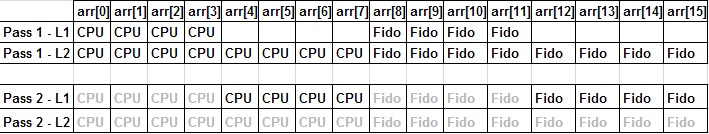
\includegraphics[width=0.8\textwidth]{FidoExample.jpg}
\caption{Visual representation of requests in the two phases: the initial miss on \textbf{arr[0]} and after the hit on \textbf{arr[0]}. Black text represents requests made while gray text represents previously completed requests. }
\end{figure}

Ideally, in the event of a cache miss, we could squash all pending cache requests in the pipeline and start with fresh requests. As our prefetcher did not have this ability, we were forced to keep a limit on how far ahead we allowed Fido to run. This was done with a hard-coded constant number of L2 cache lines we would allow the prefetcher to run ahead of the currently requested L1 line address. Across all the given traces, we found 23 to preform the best. This lookahead limit as prevented Fido from evicting cache lines that would be needed soon with data that would be needed much later (keep in mind Fido's goal is warm the L2 cache but it must bounce through L1 to do so).

Lastly, Fido required a \textit{ready} flag. The \textit{ready} flag allows our prefetcher to retry a requested address in event the L2 queue is full. Once the next request was calculated, the \textit{ready} flag was to true. Only once the request was added to the L2 queue, was \textit{ready} flag set to false. While in the ready state, the prefetcher would not attempt to calculate any new requests and would instead remain idle until the last request had be successfully submitted. The prevented the prefetcher from overrunning the L2 queue with new requests and allowed the CPU to insert new requests in the pipeline.

\subsection{Trial And Error}
As Fido relies on a number of constants to reduce overall state, we experimented with a few different values of the number of L2 lines we allowed as lookahead. Using the Newtonian method we started with 10 and kept increasing by 10 until we saw worse performance. At that point we divided the step in half and re-evaluated eventually settling on 23 for the \textit{look-ahead} constant. Certain values improved performance for some traces, while hindering others. 23 seemed to be well balanced between the how much it helped some traces and how much it hurt others.  

\section{State Accounting}
Fido is less than 4 bytes in size and consists of one next-to-be-requested address and the ready flag. As we always drop the 4 least significant bits fo the 32 bit address address, which calculates the L1 block we are in, and only need 1 bit to store the ready flag, this means the total state required is 29 bits. In C++, this is represented in 5 bytes. One \textit{u\_int32\_t} and a \textit{bool}. 

The \textit{look-ahead} constant does not contribute to the overall state as this value is hard-coded and cannot change. 

\section{Graphs}
Figure \ref{AMAT} summarizes AMAT results for various \textit{look-ahead} constants verses execution without any prefetcher. In all cases we see significant improvement with Fido verse execution without. 

\begin{figure}[H]

\centering
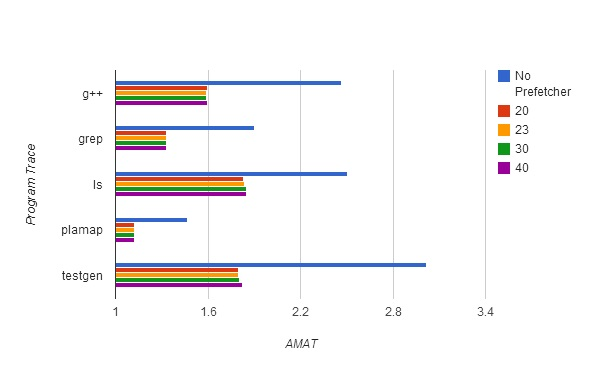
\includegraphics[width=0.9\textwidth]{AMAT.jpg}
\caption{ \label{AMAT} Comparison of Average Memory Access Time using multiple lookahead constants as well as execution without any prefetcher at all }
\end{figure}

Figure \ref{TotCyl} looks at how many cycles total a program took to complete execution for different \textit{look-ahead} constants. Even with a bad AMAT, a program could still execute in reasonable time if it had very few cycles. 
\begin{figure}[H]

\centering
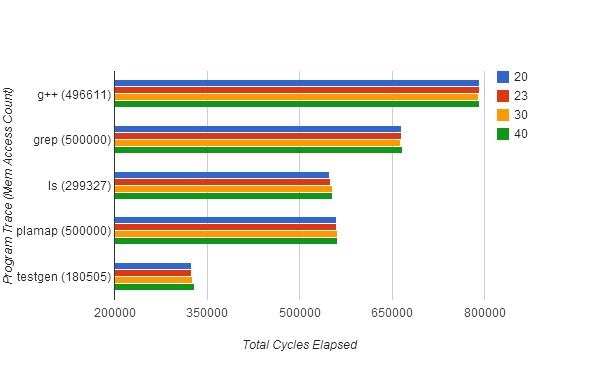
\includegraphics[width=0.9\textwidth]{TotalCycleExecuted.jpg}
\caption{ \label{TotCyl} Comparison the total number of cycles for a given trace at a given \textit{look-ahead} constant. This was calculated using the AMAT multiplied by total number of instructions executed per trace. The vertical axis gives the total memory accesses count for a given trace in parentheses}
\end{figure}



Figure \ref{speedup} summarizes the speedup using Fido and executing without any prefetcher at all for different \textit{look-ahead} constants.  
\begin{figure}[H]

\centering
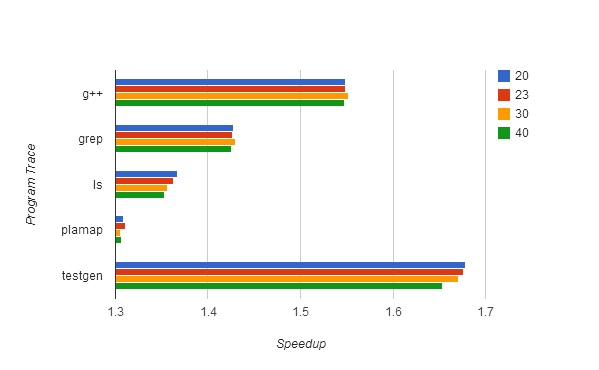
\includegraphics[width=0.9\textwidth]{SpeedupFromNoPrefetcher.jpg}
\caption{ \label{speedup} Speedup using Fido over using no prefetching at all for different \textit{look-ahead} constants}
\end{figure}

\section{Results}
As we can see from the graphs, the various \textit{look-ahead} constants between 20 and 40 all preform relatively the same varying primarily only in the third and greater significant figure. 

\begin{thebibliography}{9}

\bibitem{JouppiStreamBuff}
  Norman Jouppi,
  \emph{Improving Direct-Mapped Cache Performance by the Addition of Small Fully-Associative Cache and Prefetch Buffers}.
  Western Research Laboratory, Digital Equipment Corporation,
  1990.

\end{thebibliography}
\end{document}
